\documentclass[12pt, border=10pt]{standalone}

\usepackage{pgfplots}
\pgfplotsset{compat=1.12}

\begin{document}
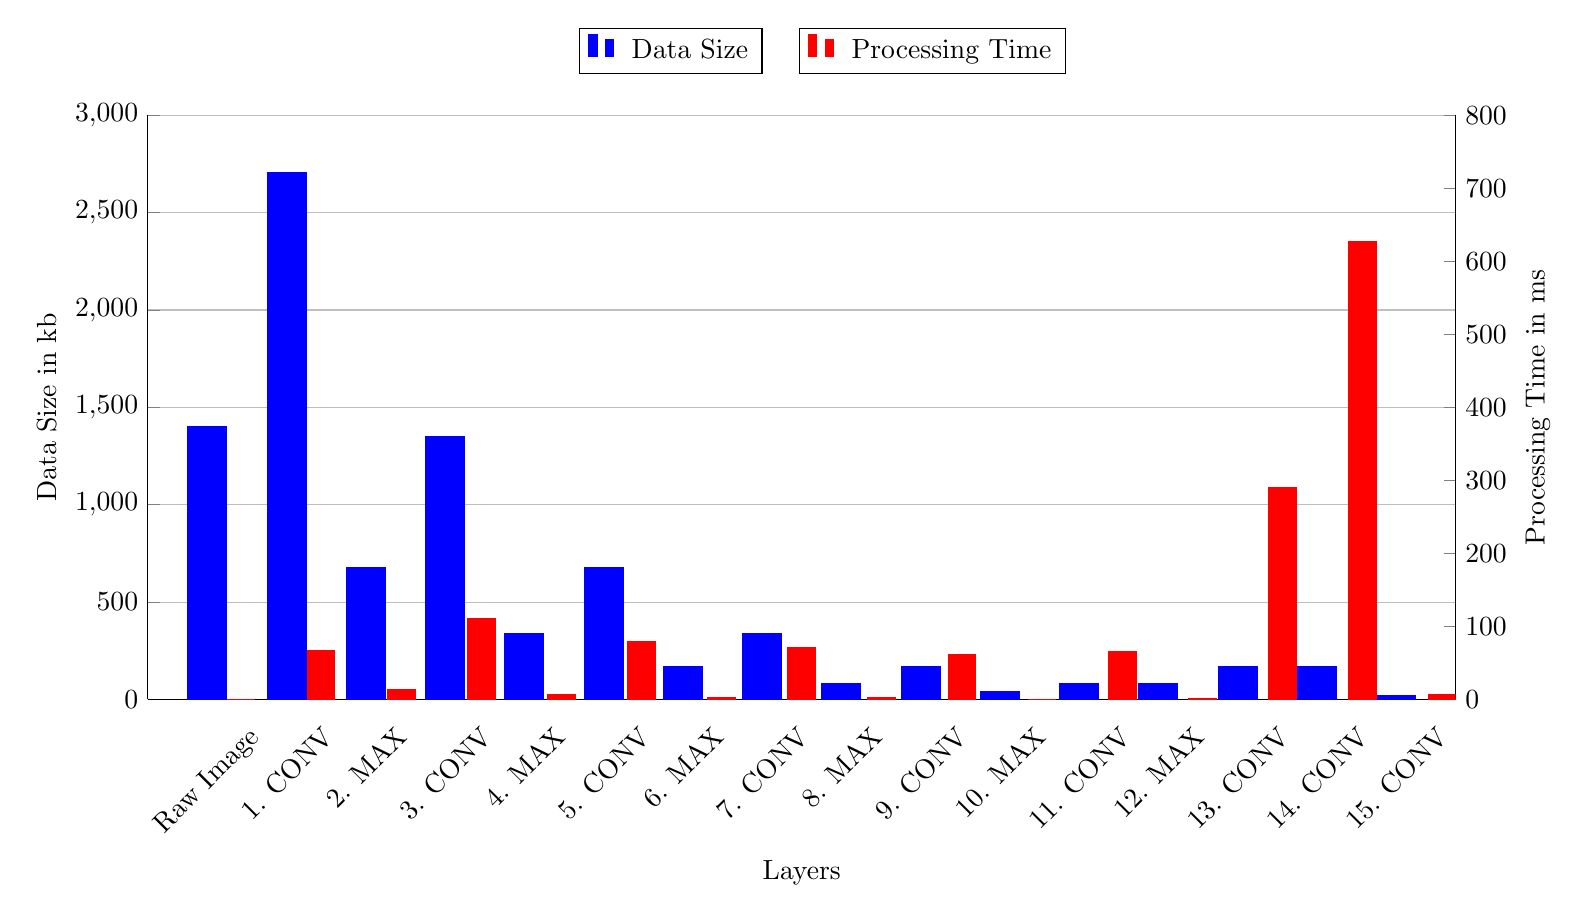
\begin{tikzpicture}
    \begin{axis}[
        width  = 1.5*\textwidth,
        axis y line*=left,
        axis x line=bottom,
        height = 9cm,
        major x tick style = transparent,
        %axis on top,
        ybar=5*\pgflinewidth,
        bar width=14pt,
        ymajorgrids = true,
        ylabel = {Data Size in kb},
        xlabel = {Layers},
        symbolic x coords={
        	Raw Image,
        	1. CONV,
        	2. MAX,
        	3. CONV,
        	4. MAX,
        	5. CONV,
        	6. MAX,
        	7. CONV,
        	8. MAX,
        	9. CONV,
        	10. MAX,
        	11. CONV,
        	12. MAX,
        	13. CONV,
        	14. CONV,
        	15. CONV
        },
        xticklabel style={rotate=45},
        xtick = data,
            scaled y ticks = false,
            enlarge x limits=0.05,
            axis line style={-},
            ymin=0,ymax=3000,
        legend columns=2,
        legend cell align=left,
        legend style={
                at={(0.4,1.15)},
                anchor=north,
                column sep=1ex
        }
    ]
       

        \addplot[style={blue,fill=blue,mark=none}]
             coordinates {
             	(Raw Image, 1400)
             	(1. CONV, 2704)
             	(2. MAX, 676)
             	(3. CONV, 1352)
             	(4. MAX, 338)
             	(5. CONV, 676)
             	(6. MAX, 169)
             	(7. CONV, 338)
             	(8. MAX, 84)
             	(9. CONV, 169)
             	(10. MAX, 42)
             	(11. CONV, 84)
             	(12. MAX, 84)
             	(13. CONV, 169)
             	(14. CONV, 169)
             	(15. CONV, 20)
             };
        \legend{Data Size}
    \end{axis}
    \begin{axis}[
    %scale only axis,
    axis y line*=right,
    axis x line=none,%axis on top,
    %xtick=\empty,
    width = 1.5*\textwidth,
    height = 9cm,
    %major x tick style = transparent,
    ybar=5*\pgflinewidth,
    enlarge x limits=0.01,
    axis line style={-},
    bar width=10pt,
    ylabel = {Processing Time in ms},
    xmin=0, xmax=16,
    scaled y ticks = false,
    ymin=-0.1, ymax=800,
    legend columns=2,
    legend cell align=left,
    legend style={
        at={(0.6,1.15)},
        anchor=north,
        column sep=1ex
    }
    ]
    \addplot[style={red,fill=red,mark=none}]
    coordinates {
    	(1,0)
    	(2, 67)
    	(3, 13)
    	(4, 111)
    	(5, 6)
    	(6, 79)
    	(7, 2)
    	(8, 71)
    	(9, 2)
    	(10, 62)
    	(11, 0)
    	(12, 66)
    	(13, 1)
    	(14, 290)
    	(15, 627)
    	(16, 7)
    };
    \legend{Processing Time}
    \end{axis}

\end{tikzpicture}
\end{document}